\chapter{System Requirement Specification}

\section{Overall Description}
The \textbf{PlateWise} platform is a modern, cloud-native web application designed to deliver real-time visual food recognition, culinary reasoning, and interactive cooking guidance. Operating on a micro-serverless decoupled architecture, the frontend client executes inside modern web browsers using React 19 and Vite, while compute-intensive operations, secure API credential management, and multi-modal neural inference are handled via Vercel Edge Serverless Functions and Groq's high-throughput LPU cloud.

This chapter outlines the system block diagram, hardware and software dependencies, detailed UML use case specifications, and the multi-tier input validation and fault-tolerance mechanisms that ensure system stability.

\section{Block Diagram / System Architecture}
The system adheres to a contemporary three-tier decoupled architecture comprising the Client Tier, Serverless Edge API Tier, and External Artificial Intelligence Infrastructure. Figure \ref{fig:blockdiagram} illustrates the complete architectural schematic and inter-module data flow.

\begin{figure}[H]
\centering
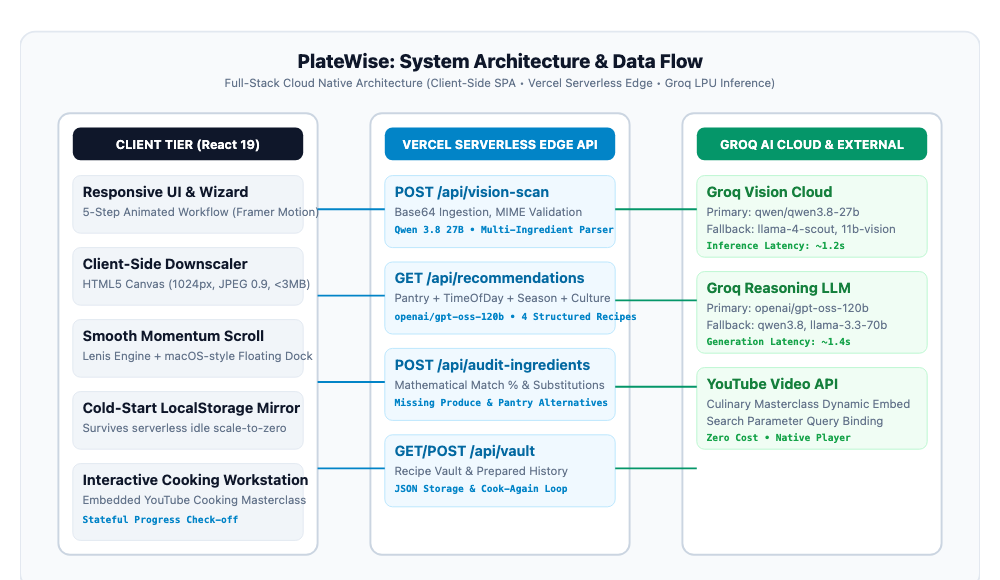
\includegraphics[width=0.95\linewidth]{images/platewise_architecture.png}
\caption{PlateWise System Architecture Block Diagram highlighting data flow between the Client SPA, Vercel Serverless Edge Functions, and Groq LPU AI Cloud.}
\label{fig:blockdiagram}
\end{figure}

\subsection*{Core Architectural Tiers}
\begin{enumerate}
    \item \textbf{Client Tier (React 19 + Vite):}
    \begin{itemize}
        \item \textbf{5-Stage Wizard Coordinator:} Manages active progression across Scan, Suggest, Audit, Cook, and Vault stages using Framer Motion spring-physics transitions.
        \item \textbf{HTML5 Canvas Pre-Processor:} Downscales raw mobile camera photographs (often 8 to 12 MB) to a maximum edge of 1024 pixels with 0.9 JPEG compression, reducing upload bandwidth by over 85\% without sacrificing visual fidelity.
        \item \textbf{Kinetic Smooth Scrolling:} Incorporates the Lenis momentum scroll library alongside an interactive macOS-style dock component.
        \item \textbf{Dual-Tier State Synchronizer:} Mirrors the active pantry and cooking history to \texttt{localStorage}, eliminating vulnerability to serverless cold-start data wipeout.
    \end{itemize}

    \item \textbf{Serverless Edge Gateway Tier (Vercel Functions in Node.js):}
    \begin{itemize}
        \item \texttt{/api/vision-scan}: Receives base64-encoded image payloads up to 10 MB, sanitizes inputs, and queries multi-modal vision models.
        \item \texttt{/api/recommendations}: Accepts dynamic query parameters (\texttt{timeOfDay}, \texttt{season}, \texttt{culture}, \texttt{inventory}) and outputs four structured recipes formatted as deterministic JSON arrays.
        \item \texttt{/api/audit-ingredients}: Evaluates recipe requirements against user inventory, calculating mathematical match percentages and culinary substitutions.
        \item \texttt{/api/vault}: Provides lightweight REST endpoints for persisting completed meal logs.
    \end{itemize}

    \item \textbf{Artificial Intelligence \& External Services Tier:}
    \begin{itemize}
        \item \textbf{Groq Multi-Modal Vision Cloud:} Executes \texttt{qwen/qwen3.8-27b} (with fallback to \texttt{meta-llama/llama-4-scout} and \texttt{llama-3.2-11b-vision}), achieving multi-ingredient extraction in $< 1.5$ seconds.
        \item \textbf{Groq High-Reasoning LLM:} Executes \texttt{openai/gpt-oss-120b} (with fallback to \texttt{llama-3.3-70b-versatile}) to synthesize detailed recipes with precise prep times, ingredients, and step instructions.
        \item \textbf{YouTube Video Embed API:} Dynamically constructs search-driven culinary video queries, embedding relevant tutorials directly into the active cooking stage without API key quotas.
    \end{itemize}
\end{enumerate}

\section{Hardware and Software Requirements}

\subsection*{Client-Side Requirements}
\begin{itemize}
    \item \textbf{Device:} Any modern smartphone, tablet, laptop, or desktop computer.
    \item \textbf{Browser:} Google Chrome 105+, Mozilla Firefox 100+, Apple Safari 16+, or Microsoft Edge 105+ with JavaScript enabled.
    \item \textbf{Input Hardware:} Integrated camera or standard file system access for image upload.
    \item \textbf{Network:} Standard 3G/4G/5G mobile data or broadband connection ($> 1$ Mbps).
\end{itemize}

\subsection*{Development and Serverless Environment Requirements}
\begin{itemize}
    \item \textbf{Operating Environment:} Node.js version 20.x or higher (LTS).
    \item \textbf{Frontend Bundler:} Vite 8.x with React 19.x and TailwindCSS 4.x.
    \item \textbf{Hosting Platform:} Vercel Serverless Edge Network (Max duration: 30s per invocation, 1024 MB memory allocation).
    \item \textbf{AI Acceleration:} Groq LPU (Language Processing Unit) Cloud API with authorized API access keys.
\end{itemize}

\section{Use Case Diagram and Specifications}
The functional capabilities of the PlateWise platform are illustrated via the UML Use Case Diagram in Figure \ref{fig:usecase}.

\begin{figure}[H]
\centering
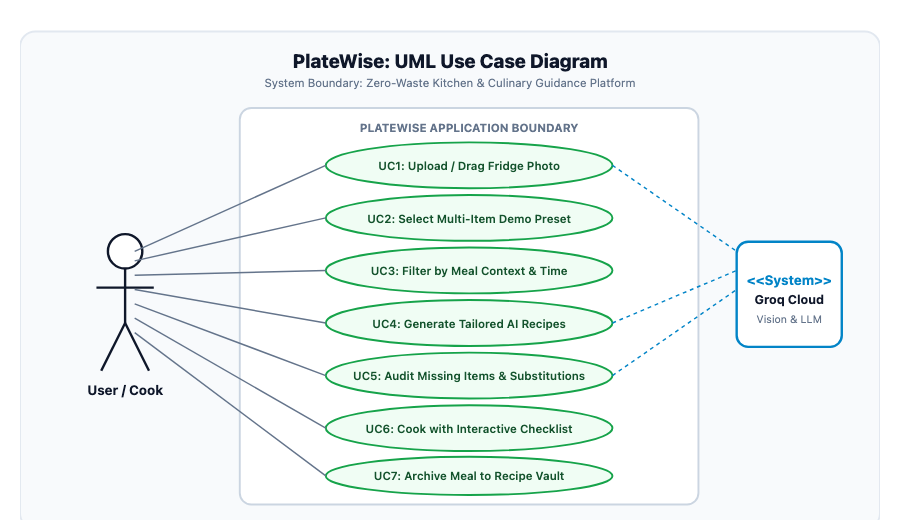
\includegraphics[width=0.90\linewidth]{images/platewise_usecase.png}
\caption{UML Use Case Diagram showing user interactions across visual scanning, contextual recommendation, ingredient auditing, cooking, and meal archiving.}
\label{fig:usecase}
\end{figure}

\subsection*{Use Case Descriptions}
\begin{itemize}
    \item \textbf{UC1 (Upload / Drag Fridge Photo):} The user drops a photo or uses their smartphone camera to submit an image of their refrigerator. The client downscales the image and submits it to \texttt{/api/vision-scan}.
    \item \textbf{UC2 (Select Multi-Item Demo Preset):} The user selects one of three verified multi-ingredient presets (\textit{Stocked Fridge}, \textit{Countertop Prep}, or \textit{Market Basket}) to instantly test full-inventory extraction with a single click.
    \item \textbf{UC3 (Filter by Meal Context):} The user configures meal parameters (Breakfast/Lunch/Dinner, Monsoon/Summer/Winter, Indian Comfort/Continental) to guide recipe generation.
    \item \textbf{UC4 (Generate Tailored AI Recipes):} The system invokes Groq's high-reasoning LLM to synthesize four contextual recipes tailored to the available inventory.
    \item \textbf{UC5 (Audit Missing Items \& Substitutions):} The system computes a match score ($0\%$ to $100\%$), identifies missing items, and provides culinary substitutes (e.g., Greek yogurt for heavy cream).
    \item \textbf{UC6 (Cook with Interactive Checklist):} The user follows step-by-step instructions with an embedded YouTube tutorial video and interactive check-off items.
    \item \textbf{UC7 (Archive Meal to Recipe Vault):} The user marks the meal as cooked, permanently recording the preparation timestamp and details in the recipe vault.
\end{itemize}

\section{End-to-End Processing Pipeline}
Figure \ref{fig:pipeline} depicts the sequential pipeline executed across the five stages of the wizard.

\begin{figure}[H]
\centering
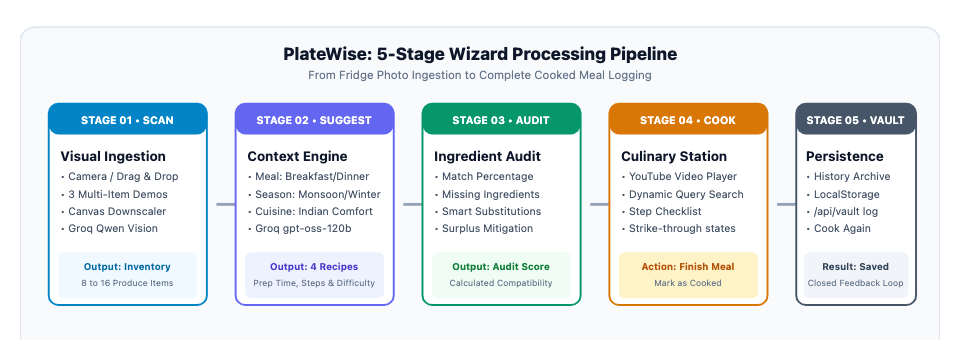
\includegraphics[width=0.95\linewidth]{images/platewise_flowchart.png}
\caption{PlateWise 5-Stage Wizard Processing Pipeline from photo input to recipe vault archiving.}
\label{fig:pipeline}
\end{figure}

\section{Input Validation and Fault Tolerance}
To guarantee enterprise reliability on serverless architectures, PlateWise incorporates four defensive validation layers:
\begin{enumerate}
    \item \textbf{MIME Type \& Payload Bounds Verification:} The serverless gateway rejects any upload lacking a valid \texttt{image/jpeg}, \texttt{image/png}, or \texttt{image/webp} signature. Payloads exceeding 10 MB are rejected before consuming memory.
    \item \textbf{Client-Side Canvas Sanitization:} The browser pre-processor scales large photos to a max 1024px boundary and normalizes EXIF orientation, preventing memory exhaustion on edge nodes.
    \item \textbf{Candidate Vision Fallback Cascade:} If the primary vision model (\texttt{qwen/qwen3.8-27b}) experiences transient rate limiting or downtime, the handler automatically catches the exception and reroutes the base64 payload to \texttt{meta-llama/llama-4-scout-17b} and \texttt{llama-3.2-11b-vision-preview}.
    \item \textbf{Deterministic JSON Schema Enforcing:} LLM prompts enforce strict JSON object extraction. If the model outputs conversational preamble, custom regex extractors isolate the bracketed JSON array, guaranteeing zero UI rendering crashes.
\end{enumerate}
